%%%%%%%%%%%%%%%%%%%%%%%%%%%%%%%%%%%
%%  Webseite / Front end
%%%%%%%%%%%%%%%%%%%%%%%%%%%%%%%%%%%
\section{Analyse front end}

Die Webseite der Wetterstation Arbon besteht neben der Homepage aus zwölf Unterseiten. Für uns wichtig sind all jene, die mit den Sensordaten, der Webcam, oder der Datenbank in Verbindung stehen. (hervorgehoben in Abb.\ref{img:sitemap}). Im folgenden werden diese Seiten und deren Probleme genauer erläutert.

\begin{figure}[h!]
	\centering
	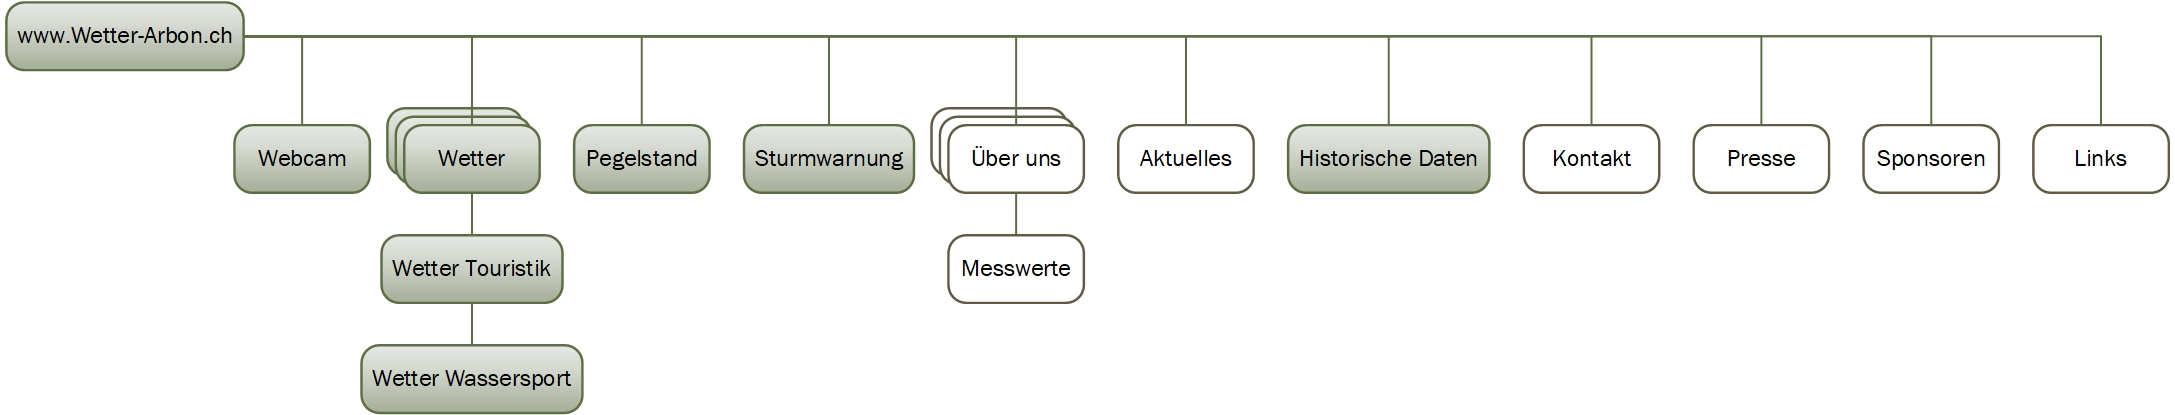
\includegraphics[width=0.9\linewidth]{img/sitemap2}
	\caption{Sitemap der Webseite}
	\label{img:sitemap}
\end{figure}


% ################################
% Problem Adobe Flash
% ################################
\subsection{Browser-Kompatibilität}
\label{subsec:flash}
Der Wettertransmitter sendet seine Daten über eine RS-484 Schnittstelle. Die Software \textit{Weather Display} \footnote{ \url{http://www.weather-display.com}} verarbeitet diese Daten und stellt sie als Text-Files für andere Anwendungen zur Verfügung. Die Zusatzsoftware \textit{Weahter Display Live} (WDL) \footnote{ \url{http://www.weather-display.com/wdlive}} liest nun eben dieses Text-File ein, und erstellt damit eine Adobe Flash Animation, wie in Abbildung~\ref{img:responsive} dargestellt (gelb markiert).

% Problem Flash
\subsection*{Problem}
Adobe Flash war eine einfache Möglichkeit animierte Grafiken auf Webseiten darzustellen und wurde praktisch von allen Browsern, nach Installation des Plug-ins, unterstützt. Diverse Sicherheitslücken und der Umstand, dass es sich um eine proprietäre d.h. closed-source Software handelte, führten dazu, dass Apple 2010 entschied Adobe Flash auf ihrem Mobile-Betiebsystem \textit{iOS} nicht mehr zu unterstützen\cite{Apple:ThoughtsOnFlash}. Sämtliche Adobe Flash Animationen können somit nicht auf iPhone und iPad angezeigt werden. Da ein Grossteil der Schweizer Bevölkerung jedoch genau diese Mobilgeräte verwendet, wurde für die Wetterstation folgender Workaround geschaffen: Der Browser prüft zuerst, ob das Gerät Adobe Flash unterstützt. Wenn ja wird die normale Applikation geladen, wenn nicht wird ein Printscreen der Applikation geladen. Der Nachteil dieses Workarounds ist jedoch, dass der Printscreen weder dynamisch noch interaktiv ist. Um die aktuellen Werte zu erhalten muss die Seite jeweils neu geladen werden. Die interaktiven Elemente sind unbrauchbar d.h. die Änderung von Einheiten, Anzeige von Rekordwerten und weiteren Graphen ist nicht möglich. Im Juli 2017 hat Adobe zudem angekündigt, dass Adobe Flash im Jahr 2020 eingestellt wird\cite{Adobe:FlashTheFutureofInteractiveContent}.

% Lösung Flash
\subsection*{Lösungsansatz}
2014 wurde die neue HTML-Spezifikation, HTML5, fertiggestellt. HTML5 bietet diverse neue Funktionen unter anderem im Bereich dynamischer Grafiken. HTML5 ist der neue Web-Standard und wird von allen modernen Web-Browsern unterstützt. Es gibt diverse Javascript-Bibliotheken wie zum Beispiel Google Charts\footnote{ \url{https://developers.google.com/chart/interactive/docs/gallery}} oder D3.js\footnote{ \url{https://github.com/d3/d3/wiki/Gallery}}, die auf die Darstellung von Daten spezialisiert sind. HTML5 eignet sich somit ideal als Ersatz von Adobe Flash um die Wetterdaten grafisch darzustellen. 


% ################################
% Semantisches Web
% ################################
\subsection{Semantisches Web}
Weather Display Live ist eine vorgefertigte Software, die nur sehr eingeschränkt angepasst werden kann. Die Art und Anordnung der Anzeigeinstrumente kann beispielsweise frei bestimmt werden. Viel mehr geht nicht.

\subsection*{Problem}
Auf sehbehindert Menschen, oder Menschen mit anderen Beeinträchtigungen kann keine Rücksicht genommen werden. Es kann weder Farbe noch Schriftgrösse angepasst werden. Die Adobe Flash Applikation unterstützt auch kein Vorleseprogramm, wie es sehbehinderte Menschen verwenden.

\subsection*{Lösungsansatz}
Mit HTML5 gibt es diverse Möglichkeiten für die semantische Auszeichnung des Webseiteninhalts. Dies ermöglicht es die Webseite oder zumindest Teile davon barrierefrei zu gestalten und so mehr Menschen den Inhalt zugänglich zu machen.



% ################################
% Problem Responsive Design
% ################################
\subsection{Responsive Design}
Die Webseite der Wetterstation ist mit dem Content-Management-System (CMS) \textit{Openfile64Light} der Firma Screenbox\footnote{ \url{https://www.screenbox.net}}  erstellt. Dieses unterstützt grundsätzlich responsive Design. Das CMS gibt den Rahmen der Webseite vor. Spezielle Inhalte wie zum Beispiel die Adobe Flash Animation werden als sogenannte Applikationen behandelt und in die Seite eingebettet, gelb markiert in Abbildung~\ref{img:responsive}, links.

\begin{figure}[h!]
	\centering
	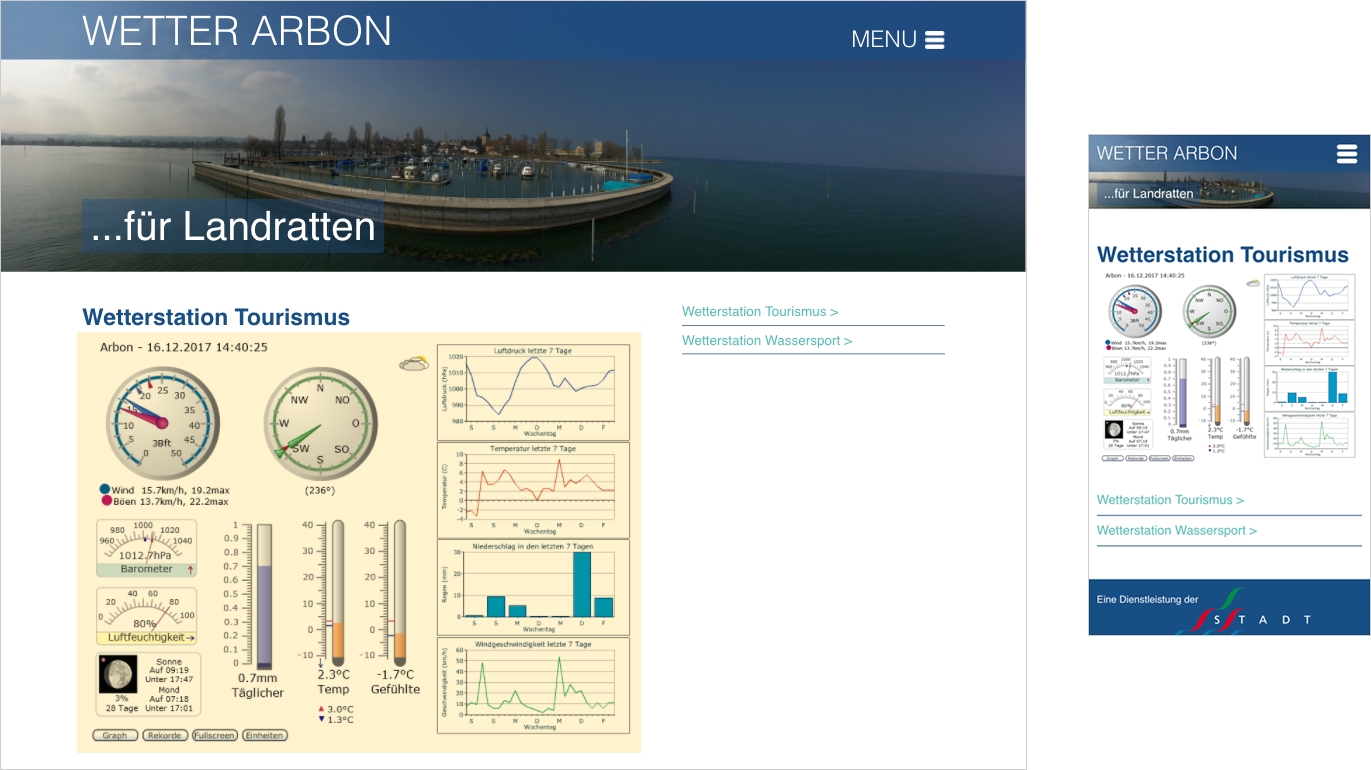
\includegraphics[width=1\linewidth]{img/responsive}
	\caption{Responsive Design: Vergleich Desktop und Mobile}
	\label{img:responsive}
\end{figure}


\subsubsection*{Problem}
Unterstützt die eingebettete Applikation kein responsive Design, so wird dieser Teil einfach linear skaliert. Dies führt dazu, dass die Anzeige der Wetterstationsdaten auf einem Mobilgerät kaum mehr lesbar sind, wie in Abbildung~\ref{img:responsive}, rechts dargestellt.


\subsubsection*{Lösungsansatz}
Mit der Adobe Flash Applikation lässt sich dieses Problem nicht lösen. Da aber, wie in Abschnitt~\ref{subsec:flash} erklärt, die Adobe Flash Applikation ohnehin abgelöst werden muss, wird bei der Ausarbeitung der neuen Anzeige darauf geachtet, dass die Wetterdaten auf allen gängigen Geräten problemlos lesbar sind. Da davon auszugehen ist, dass die Webseite häufig von Mobilgeräten aus betrachtet wird, wird das Designkonzept \textit{mobile first} angewendet. Das bedeutet, dass zuerst die Mobile-Seite designt wird und anschliessend die Desktop-Seite, inhaltlich gesehen somit vom Wichtigen zum weniger Wichtigen. 



% ################################
% Problem Graphen
% ################################
\subsection{Darstellung der Wetterdaten}
Insesondere für Segler ist der Verlauf der Wetterdaten interessant zum Beispiel der Verlauf der Windgeschwindigkeit. Auf der Webseite werden deshalb neben den aktuellen Wetterdaten ausgewählte Wetterdatenverläufe dargestellt, wie in Abbildung~\ref{img:responsive} ersichtlich. Bei diesen Grafiken geht es primär um die Tendenz und nicht um die Absolutwerte.

% Windgeschwindigkeit
\subsubsection*{Problem: Automatische y-Skalierung von Graphen}
Die Skalierung der y-Achse wechselt automatisch je nach Windstärke wie Abbildung \ref{img:wind-geschw} zeigt. Das Problem ist, dass ein schnelles Ablesen der Anzeige nicht möglich ist, da immer zuerst die y-Skalierung angeschaut werden muss, was mühsam ist.

\begin{figure}[h!]
	\centering
	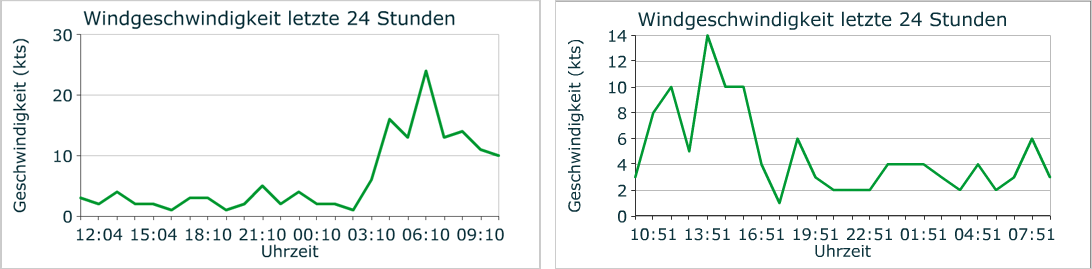
\includegraphics[width=1\linewidth]{img/wind-geschw}
	\caption{Anzeige der Windgeschwindigkeit mit variabler y-Skalierung}
	\label{img:wind-geschw}
\end{figure}

% Windrichtung
\subsubsection*{Problem: Sprung in der Windrichtungsanzeige}
Der zeitliche Verlauf der Windrichtung wird als Linie in einem xy-Graphen dargestellt. Die y-Achse geht von 0 Grad bis 360 Grad. Das Problem bei dieser Darstellung ist, dass wenn der Wind über Norden dreht dies als Sprung in der Grafik abgebildet wird, wie in Abbildung~ \ref{img:wind-richtung} dargestellt. Auf Grund des Verlaufs der letzten sieben Tage ist davon auszugehen, dass die Darstellung vom Mitwoch falsch ist. Durch die Interpolation der Werte entsteht so eine verwirrende und falsche Aussage.

\begin{figure}[h!]
	\centering
	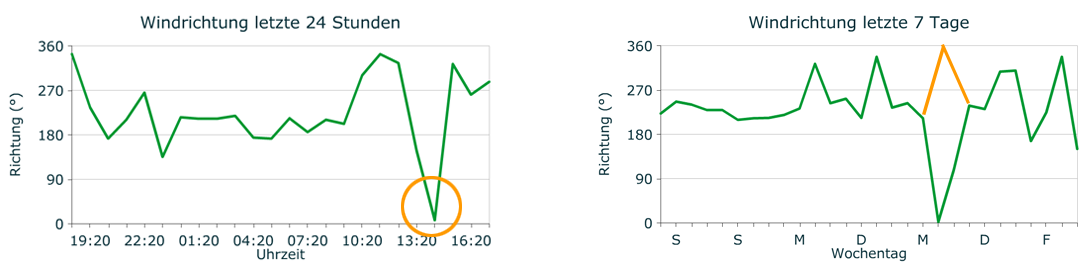
\includegraphics[width=1\linewidth]{img/wind-richtung}
	\caption{Anzeige der Windrichtung}
	\label{img:wind-richtung}
\end{figure}

\subsubsection*{Lösungsansatz}
Bei der Erstellung der neuen Anzeige wird darauf geachtet, dass die Graphen auf den ersten Blick eine klare Aussage zulassen indem fixe y-Skalierungen verwendet werden. Die Auswahl der Darstellungsart erfolgt zudem so, dass keine Missverständnisse bzw. Falschaussagen entstehen.



% ################################
% Problem Sturmwarnung
% ################################
\subsection{Sturmwarnung}
\label{subsec:sturmwarnung}
Auf dem Bodensee gibt es einen Sturmwarndienst, der die Schiffsführer vor aufkommendem Sturm warnen soll. Der Sturmwarndienst wird vom Deutschen Wetterdienst in Zusammenarbeit mit MeteoSchweiz betrieben. Rund um den Bodensee sind dafür über 60 Sturmwarnleuchten installiert (Abbildung \ref{img:sturm2}). Diese blinken 40 mal pro Minute bei Windböen  über 25 Knoten und 90 mal pro Minute bei Windböen über 34 Knoten. Die aktuelle Warnsituation wird zudem auf der Webseite der Kantonspolizei Thurgau\footnote{ \url{http://www.kttg.ch/kapo/htm/stwarn.shtml}} als Bild, siehe Abbildun~\ref{img:sturm} rechts, publiziert. Dieses Bild wurde bis im September 2017 auf der Webseite der Wetterstation direkt eingebunden.

\begin{figure}[h!]
	\centering
	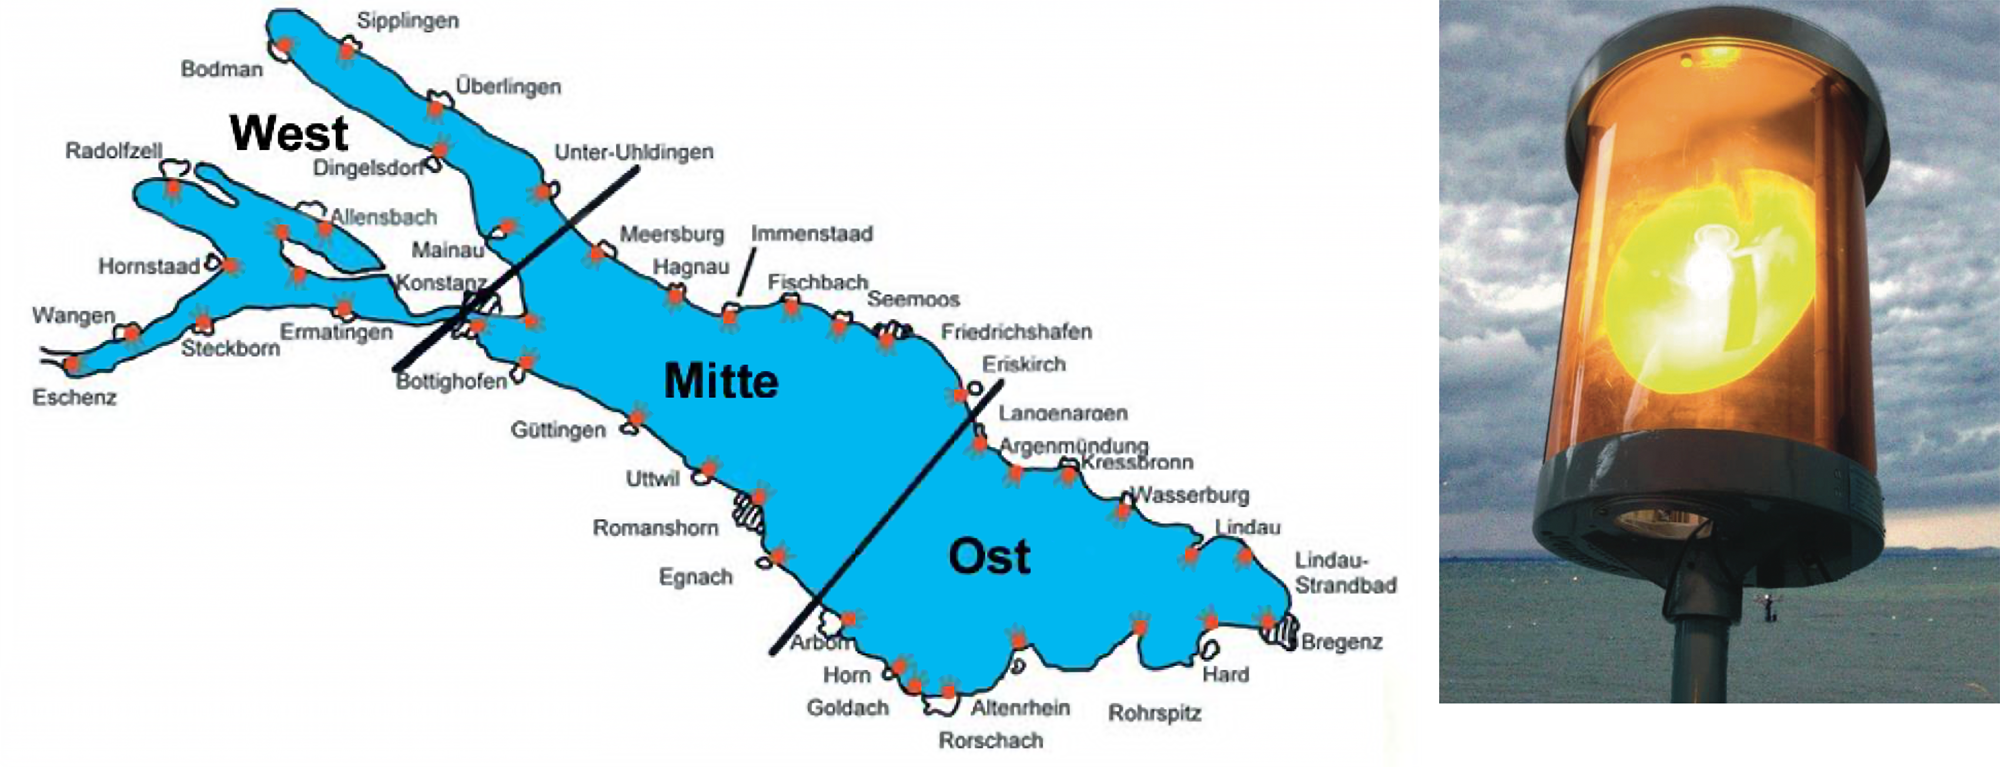
\includegraphics[width=1\linewidth]{img/sturm2}
	\caption{Sturmwarndienst Bodensee}
	\label{img:sturm2}
\end{figure}


\subsubsection*{Problem: HTTP}
Die Webseite der Kantonspolizei Thurgau kann nur über eine unverschlüsselte HTTP-Verbindung aufgerufen werden. Die verschlüsselte Verbindung über HTTPS wird nicht unterstützt. Google Chrome und Mozilla Firefox planen HTTP-Seiten zukünftig abzuwerten und mit einer Warnung als \flqq nicht sicher\frqq zu markieren\cite{Chromium:marking-http-as-non-secure}\cite{Mozilla:DeprecatingNon-SecureHTTP}. Für normale User ist diese Meldung nicht verständlich und erzeugt ungewolltes Misstrauen in die Webseite. 
Seit 2014 verwendet Google zudem HTTPS als Ranking Signal. Bisher war es ein sehr schwaches Signal d.h. die Gewichtung lag bei unter einem Prozent. Google behält sich allerdings vor, die Gewichtung zu erhöhen\cite{Googleblog:https-as-ranking-signal}. Webseiten, die nicht über HTTPS verfügen werden somit in der Trefferliste weiter unten angezeigt. 
Aus diesen beiden Gründen hat Screenbox im Herbst 2017 alle Kunden aufgefordert ihre Webseiten auf HTTPS umzustellen. Die Webseite der Wetterstation Arbon konnte problemlos umgestellt werden - mit einer Ausnahme: Da die Sturmwarnung direkt eingebettet war, konnte die Sturmwarnung-Seite der Wetterstation Arbon nicht auf HTTPS umgestellt werden. Als Sofortmassnahme wurde deshalb das eingebettete Bild entfernt und durch einen Link auf die Webseite der Kantonspolizei ersetzt, siehe Abbildung~\ref{img:sturm} links. Das dies keine langfristige Lösung sein kann, versteht sich von selbst.

\begin{figure}[h!]
	\centering
	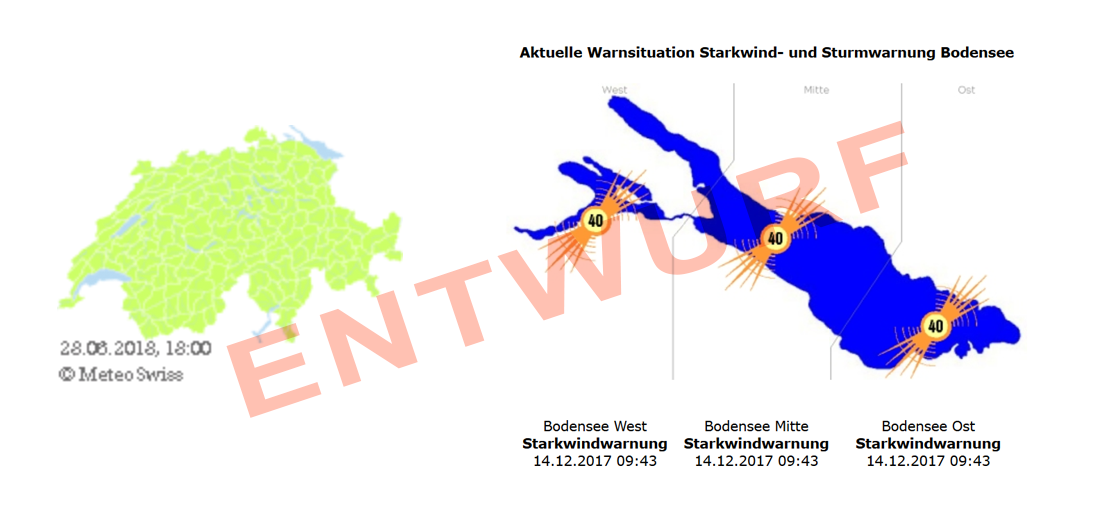
\includegraphics[width=1\linewidth]{img/sturm}
	\caption{}
	\label{img:sturm}
\end{figure}

\subsubsection*{Problem: Warnzeiten}
Der Sturmwarndienst wie in Abschnitt \ref{subsec:sturmwarnung} beschrieben, ist kein 24h-Service. Der Dienst ist nur während den folgenden Warnzeiten\footnote{ \url{https://kapo.tg.ch/public/upload/assets/56408/A5\%20Sturmwarnung.pdf}} aktiv:

\begin{itemize}  
\item 1. April - 31. Oktober: 06:00 - 22:00 Uhr 
\item 1. November - 31. März: 07:00 - 20:00 Uhr
\end{itemize}

Ein durchgehender Service wäre im Hinblick auf die Sicherheit auf dem See wünschenswert.

\subsubsection*{Lösungsansatz}
Die Information zum Sturmwarndiest des Bodensees sollen durch eine API-Anfrage implementiert und selbst dargestellt werden. Ob weiterhin das offizielle Signal für die Sturmleuchten, oder ein 24h-Service zum Beispiel von MeteoSchweiz verwendet werden soll, muss während der Bachelor-Arbeit mit dem Auftraggeber geklärt werden.



%
%\subsection{Probleme summiert}
%\Diskussionspunkt{
%\begin{itemize}  
%\item Flash Weiterentwicklung wird gestoppt und schon von vielen Geräten nicht mehr Unterstützt
%\item Screenshots der aktuellen Verhältnissen nicht optimal
%\item Die Skalierung der Graphen ist mehr verwirrend als hilfreich
%\item Der HTTP standard ist unsicher, wird in Zukunft eingestellt
%\end{itemize}
%}
%\sout{Das Problem der Webseite und vor allem der beiden Applikationen ist, dass viele Geräte Flash nicht mehr oder in naher Zukunft nicht mehr unterstützen. Zusätzlich ist die Lösung mit dem Screenshot der aktuellen Verhältnisse auch keine optimale Lösung. Auch sind die Schreibfehler, welche entdeckt wurden bei näherer Betrachtung auch nicht Vorteilhaft. Weiter ist die Wetterapplikation nicht nach dem Prinzip responsive Design aufgebaut, welches in der heutigen Zeit ein wichtiger Bestandteil einer Webseite ist. Zusätzlich zum Flash, von der Gebrauch gemacht wird sind die Anzeigen auf der Touristik bzw. Wassersport Seite unschön. }
%
%
%\subsection{Lösungsansatz}
%Um die Webseite auf den neusten Stand der Technik zu bringen sollten folgende Änderungen durchgeführt werden.Die Flash-Software wird ausgemustert und die Applikation wird auf HTML5 und Javascript umgestellt. Die Webseite soll zudem im responsive Design entwickelt werden, damit auch auf mobilen Geräten die aktuelle Wetterlage sichtbar ist. Die dynamischen, sowie auch die teilweise statischen Anzeigen, werden wo möglich mithilfe der Javascript Bibliothek D3.js oder Google Charts erstellt, hiermit lassen sich ansehnliche und moderne Grafiken erstellen. Die Grafiken, sollten so gestaltet sein das auch Sehbehinderte Personen erkennen wie das Wetter momentan ist. Das heisst beispielsweise, dass die Farben auch für Farbenblinde unterscheidbar sein sollten oder blinde Personen anhand eines Vorleseprogramms erkennen wie das Wetter ist. Ein weiterer Punkt ist die Auswahl der Einheiten, diese sollen nach dem ersten Besuch gespeichert bleiben beim Client mithilfe von Webstorage.
